%----------------------------------------------------------------------------------------
%	SOLUTION 1.a
%----------------------------------------------------------------------------------------
\subsection*{CSP Problem: Cryptarithm}
The solution is shown in Fig.~\ref{fig:csp_mrv}. The \textit{Step} column shows the action performed in that step and the values obtained for each variable after taking that action is tabulated in the subsequent columns. \textit{Failure Detected} column shows if any inference results into any constraint violation, \textit{Constraint violated} column shows which constraints cause the failure, \textit{Backtrack to Step} column shows the step number where the solver backtracks if any failure happens. Once it backtracks, the solver tries other actions different from the one that resulted into the failure. Once we get the values for each variable satisfying all the constraints, we achieve a solution. \textit{Is Solution} column dictates whether an action results into a solution.
%%%%%%%%%%%%%%%%%%%%%%% ADABOOST ERROR %%%%%%%%%%%%%%%%%%%%%
\begin{figure}[!h]
	\centering
	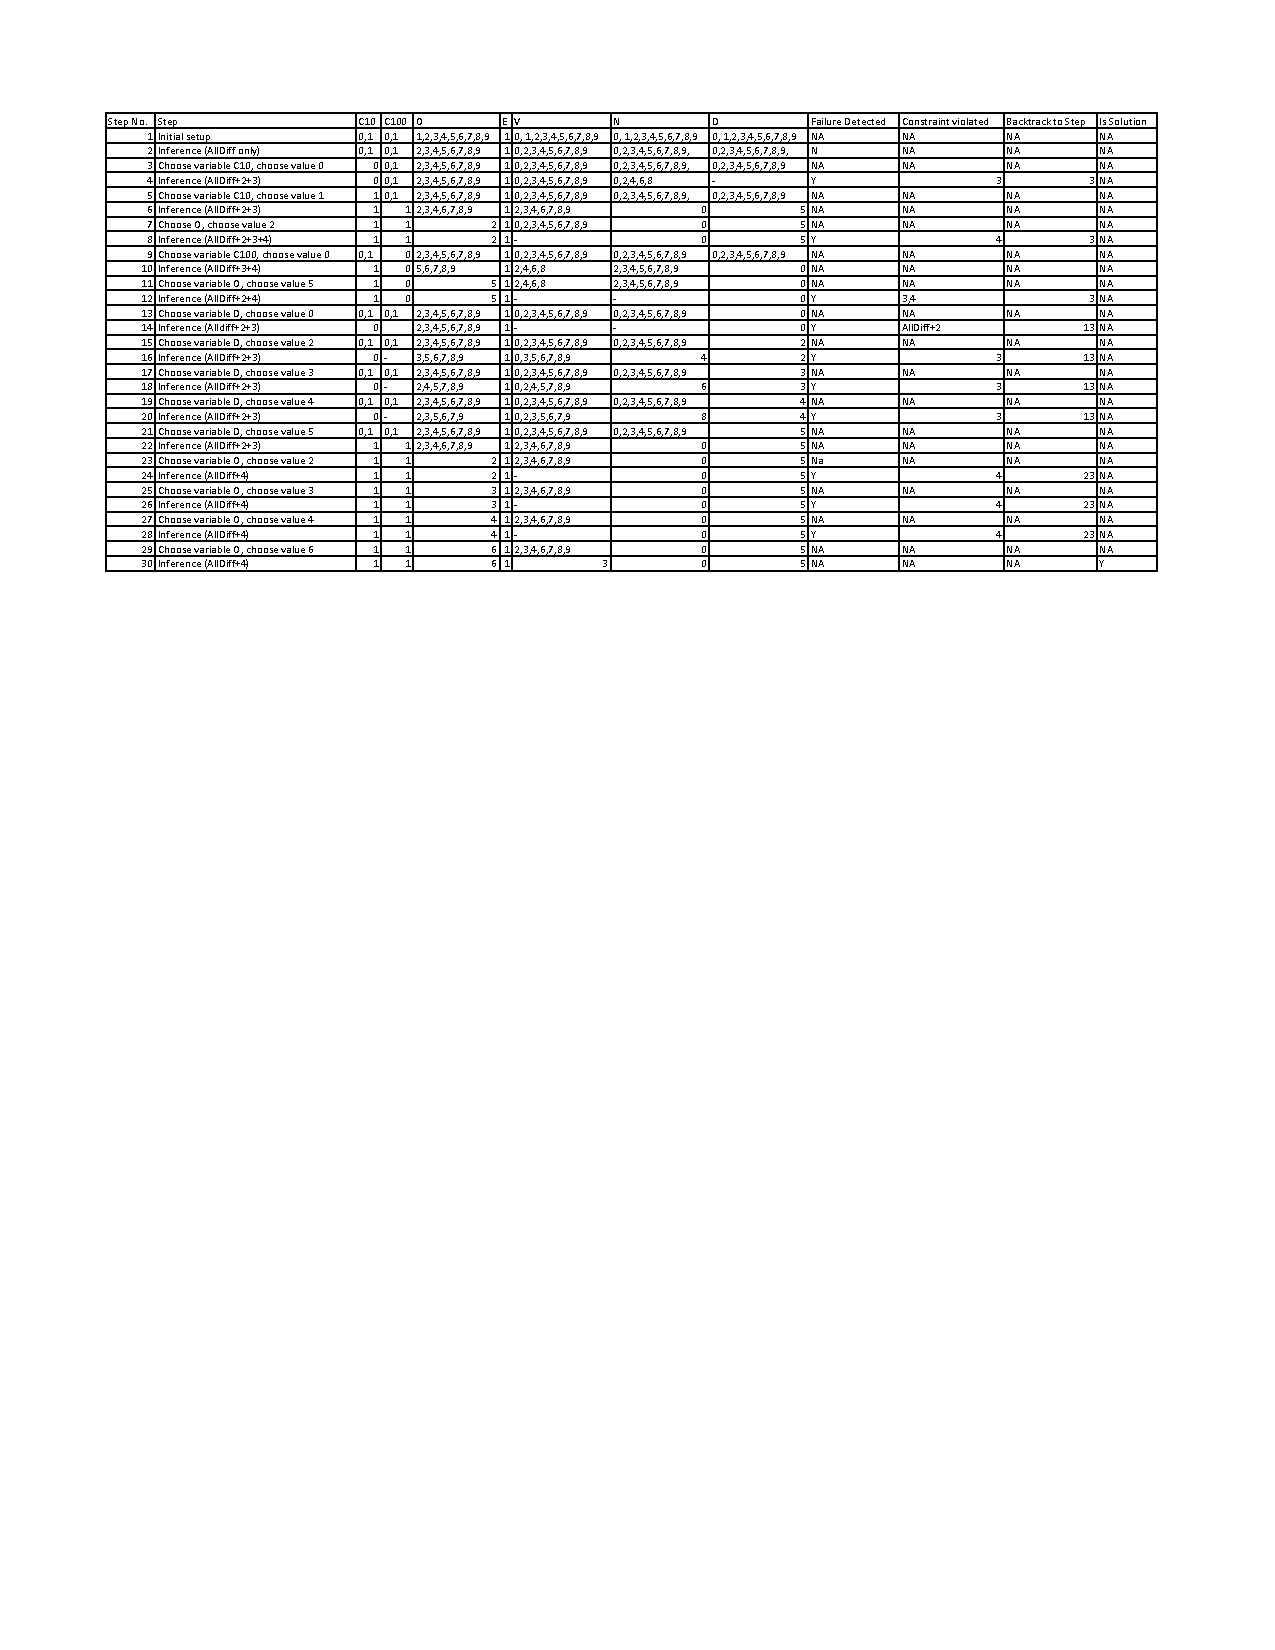
\includegraphics[angle=0,scale=1.0,trim={1.5cm 18cm 2cm 1.5cm},clip]{./csp_mrv.pdf}
	\caption{CSP: Cryptarithm Solution Step}
	\label{fig:csp_mrv}
\end{figure}

The solution I have achieved is:
\begin{table}[!h]
	\renewcommand{\arraystretch}{1.2}
	\centering
	\caption{Solution}
	\label{tbl:b_savings}
	\begin{tabular}{cccc} 
		\hline
		&$6$&$6$&$5$\\
		+&$6$&$6$&$5$\\
		\hline
		$1$&$3$&$1$&$0$\\
		\hline
	\end{tabular}
\end{table}